\section{对极约束}
	如前所述,对一般场景而言,两个成像平面构不成射影变换,它们服从更一般的\textbf{极几何}约束,可用一个矩阵$F$表示这种约束关系,矩阵$F$称为\textbf{基础矩阵},
	\begin{figure}[H]
		\begin{center}
			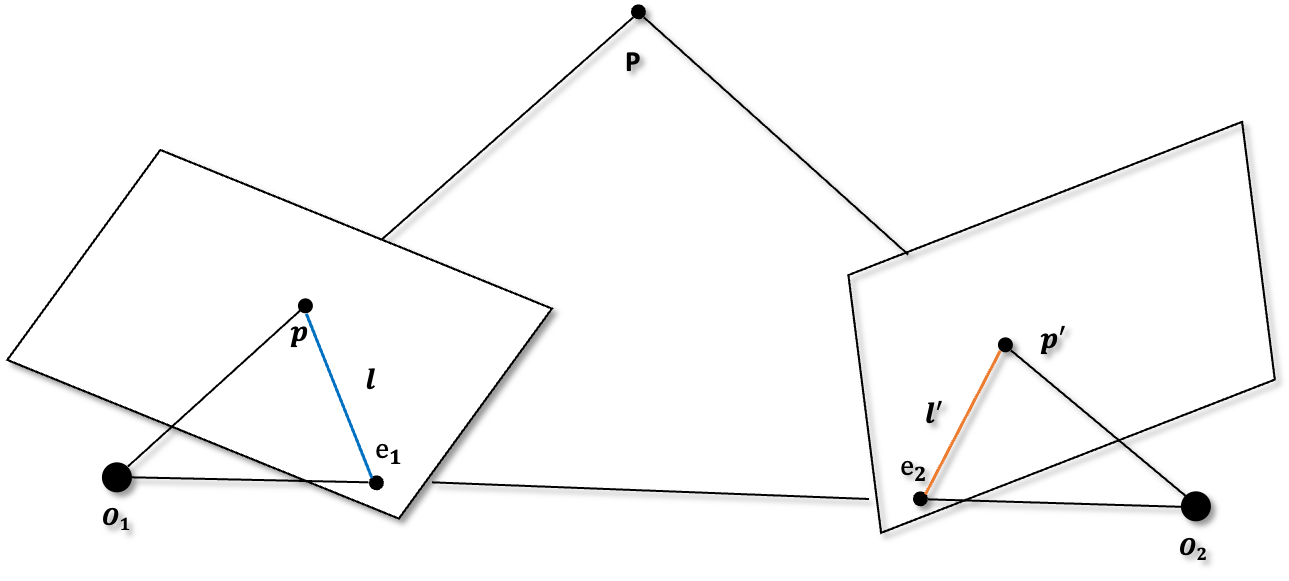
\includegraphics[width=0.8\textwidth]{../images/base_matrix.png}
		\end{center}
		\caption{两图像之间的极几何约束,$O_1,O_2$为相机\textbf{光心},$O_1O_2$为\textbf{基线},$p,p^{\prime}$为$P$在两个像素平面的像,$e,e^\prime$为\textbf{极点},$l,l^{\prime}$为\textbf{极线}}
	\end{figure}
	\begin{itemize}
		\item 世界坐标系选为第一个相机坐标系
		\item $K,K^{\prime}$是两个相机的内参矩阵
		\item $R,T$是第二个相机相对第一个相机的旋转和平移
		\item $[T]_{\times}$是$T$张成的反称矩阵,秩为$2$
		\item $e,e^\prime$为极点,$e^\prime$是$e$的投影,存在
			$$
				e^\prime =K^\prime T
			$$	
	\end{itemize}

	所有极线都过极点,所以,
	$$
		{p^\prime}^T l^\prime = 0, \quad {e^\prime}^T l^\prime = 0
	$$
	\subsection*{基础矩阵}
		$p,p^\prime$是同一个空间点$P$在两个像素平面的投影,将$p$反投影到$P$,再投影到第二个像素平面可得到$p^\prime$,根据(\ref{inverse_proj}),

		\begin{align}
			p^{\prime}_d &= K^{\prime}[R\quad T]
			\begin{bmatrix}
				dK^{-1}p\\
				1
			\end{bmatrix}\nonumber\\
			&= K^{\prime}\left(dRK^{-1}p + T\right)\nonumber\\
			&= dK^{\prime}RK^{-1}p + K^{\prime}T\label{f_inverse}\\
			&= dK^{\prime}RK^{-1}p + e^\prime\label{f_inverse_e}
		\end{align}

		尺度因子$d$在齐次坐标下并无影响,只是提醒反投影后存在一个尺度。\\

		由此可见,一般情况下$p,p^\prime$之间并非射影变换。\\

		(\ref{f_inverse_e})式两边叉乘$e^\prime$,

		$$
			p^{\prime}_d\times e^\prime = dK^{\prime}RK^{-1}p \times e^\prime
		$$

		转置一下,
		$$
			e^\prime \times p^{\prime}_d = e^\prime \times dK^{\prime}RK^{-1}p = d[e^\prime]_{\times}K^{\prime}RK^{-1}p
		$$

		两边与$p^\prime_d$作内积,
		$$
			p^\prime_d [e^\prime]_{\times}K^{\prime}RK^{-1}p = 0
		$$

		称,
		\begin{equation*}
			\mathbf{F} = [e^\prime]_{\times}K^{\prime}RK^{-1}
		\end{equation*}

		为\textbf{基础矩阵},任意点对$p^\prime,p$都满足约束,

		\begin{equation}
			{p^{\prime}}^T \mathbf{F} p = 0 \label{f_constrain}
		\end{equation}

		根据(\ref{inver_m_p}),可得到$F$的另一表达式,

		$$
			\mathbf{F} = [e^\prime]_{\times}K^{\prime}RK^{-1} = {K^{\prime}}^{-T}[T]_{\times}RK^{-1}
		$$

		下面两个表达式都是$F$的常用形式,
		\begin{align}
			\mathbf{F} &= [e^\prime]_{\times}K^{\prime}RK^{-1} \label{f_1}\\
			\mathbf{F} &= {K^{\prime}}^{-T}[T]_{\times}RK^{-1} \label{f_1}
		\end{align}

		$[T]_{\times},[e^\prime]_{\times}$的秩为2,所以$F$的秩也为2。\\

	\subsection*{点线对应}

		$p^{\prime}$在极线$l^{\prime}$上,而$p^\prime \mathbf{F} p=0$,可知,

	\begin{align*}
		l^{\prime} = Fp,\quad 
		l = F^Tp^\prime
	\end{align*}

	基础矩阵描述了点之间的约束关系,每个点对应一条极线。\\

	极点$e^\prime$也在极线$l^\prime$上,
	$$
		{e^\prime}^T l^\prime = 0 \Rightarrow {e^\prime}^TFp=0 \Rightarrow p^T F^T e^\prime = 0
	$$

	因为$p$的任意性,可知

	$$
		{e^\prime}^T F = 0, \quad Fe = 0
	$$

	沿着极线$l^\prime$搜索$p$的像,会大幅缩小搜索范围。

	\subsection*{工程实现}
		在实际计算时,通过投影矩阵的增广的投影矩阵表示更为方便,
		\begin{equation}
			N_d= M^{\prime}M^{-1} = \begin{bmatrix}
				dK^\prime R K^{-1} \quad& K^\prime T\\
				0\quad& 1\quad
			\end{bmatrix}\label{extend_f}		
		\end{equation}

		从$N_d$中截取出左上角$3\times 3$的矩阵便是旋转矩阵,右上角$3\times 1$的向量是平移向量,这在各种工具中非常容易实现。

\section{外参恢复}\label{section_recovery_outer_p}
	基础矩阵$F$包含了相机的内外参数,如果相机内参数和$F$已知,能否从$F$中分离出外参数?\\

	$$
		\mathbf{F} = {K^{\prime}}^{-T}[T]_{\times}RK^{-1} \Rightarrow {K^{\prime}}^{T}\mathbf{F} K = [T]_{\times}R = \mathbf{E}
	$$

	其中,
	$$
		\mathbf{E} = [T]_{\times}R
	$$

	称为\textbf{本质矩阵}。现在问题简化为如何从$E$中分离出外参$R,T$。\\

	根据(\ref{inverse_decompose}),$[T]_{\times}$可分解为,

	\begin{align*}
		[T]_{\times} &= U diag(1,1,0)WU^T\\
		[T]_{\times} &= U diag(1,1,0)W^TU^T
	\end{align*}

	这两种分解仅差一个尺度或者符号。$E$可表示为,

	\begin{align*}
		\mathbf{E} = U diag(1,1,0)\left(WU^TR\right)\quad 
		\text{or} \quad 
		U diag(1,1,0)\left(W^TU^TR\right)
	\end{align*}

	注意$E$是秩为2的反称矩阵,奇异值分解形式为,

	$$
		\mathbf{E} = U diag(1,1,0) V^T
	$$

	在$\mathbf{E} $确定的情况下,$U,V$是已知量,对比可知,
	\begin{align*}
		V^T = WU^TR \quad \text{or}\quad W^TU^TR
	\end{align*}

	得到$R$的两种表达式,
	\begin{align*}
		R = UW^TV^T\quad \text{or}\quad UWV^T
	\end{align*}

	$R$是旋转矩阵,所以行列式值为正,修正一下符号,

	$$
		R \leftarrow (\mathop{det} R)R
	$$

	而,
	$$
		[T]_{\times} = R^T\mathbf{E}
	$$

	这样得到$T$的反称矩阵,可以组合出$T$向量;$R$有两个值,$T$也对应有两个值。\\


	这两组解几何表示,一组场景都在相机前面;一组场景在相机后面,通过重建出的点过滤掉在后面的解即可。

\section{单应变换}

	如果拍摄场景是一张平面,法向量为$\mathbf{n}$,到原点距离为$d$,则平面方程为,
	$$
		\mathbf{n}^T P = d
	$$

	$\mathbf{n}_d = \mathbf{n}/d$,场景平面可表示为,
	
	$$
		\mathbf{n}_d^T P = 1
	$$

	像素点$p$反投影为$dK^{-1}p$,

	\begin{align*}
		p^{\prime}(d) &= K^{\prime}\left(dRK^{-1}p + T\right)\\
		&= K^{\prime}\left(dRK^{-1}p + T\mathbf{n}_d^T P\right)\\
		&= K^{\prime}\left(dRK^{-1}p + T\mathbf{n}_d^TdK^{-1}p\right)\\
		&= dK^{\prime}\left(R + T\mathbf{n}_d^T\right)K^{-1}p\\
		&= Hp
	\end{align*}

	这里的关键是第二步,代入场景平面方程,把$p$给分离了出来,$p^\prime,p$之间构成射影变换。\\

	$K^\prime$是齐次矩阵,与$dK^\prime$等价。

	\begin{equation}
		H= K^{\prime}\left(R + T\mathbf{n}_d^T\right)K^{-1} \label{homograph_matrix}
	\end{equation}

	称为\textbf{单应矩阵},因此射影变换也称为\textbf{单应变换}。\\

	$p,p^{\prime}$依然服从基础矩阵的约束,(\ref{extend_f})式的增广表示也包含了单应变换这一特殊情况。\\

	基础矩阵只是描述点与极线的对应关系,而单应矩阵描述点之间一一对应关系,这也是“\textbf{单应}”的意义。

	\subsection*{论文中的公式}

	在MVSNet中,只知道两个相机在世界坐标系的旋转和平移$R_1,t_1,R_2, t_2$,相对旋转$R$和平移$t$为,

	$$
		R = R_2R_1^{-1},\quad 
		t = t_2 - R_2R_1^{-1}t_1
	$$

	(\ref{homograph_matrix})用世界坐标系可表示为,

	\begin{align}
		H &= K_2 \left(R_2R_1^{-1} +\left(t_2 - R_2R_1^{-1}t_1\right) \mathbf{n}_d^T\right) K_1^{-1} \label{new_homograph_matrix}
	\end{align}	

	原论文中的公式是错误的,这是正确版本。\\

	增广表示蕴含了单应变换,这个复杂的式子在编程中并不会被使用到。